\lecture{2}{2. Februar 2026}{Traction, Stress, and Equilibrium}

\section{Traction, Stress, and Equilibrium}

\subsection{State of Stress} \label{sec:tracvec}
For a deformable body subject to external loading we focus on an element with area $\Delta A_n$ oriented according to the unit normal $\Vec{n}$, we call the resultant force $\Delta \Vec{F}_n$ and the resultant moment $\Delta \Vec{M}_n$.
Both are vector quanitites, and are \textit{not}, in general, parallel to $\Vec{n}$.
We represent the intensity of these as
\begin{align*}
  \lim_{\Delta A_n \to 0} \frac{\Delta \Vec{F}_n}{\Delta A_n} = \frac{\mathrm{d}\Vec{F}_n}{\mathrm{d}A_n} &= \Vec{T}_n \\
  \lim_{\Delta A_n \to 0} \frac{\Delta \Vec{M}_n}{\Delta A_n} = \frac{\mathrm{d}\Vec{M}_n}{\mathrm{d}A_n} &= \Vec{C}_n 
\end{align*}
where $\Vec{T}_n$ is known as the stress vector or the \textit{traction}, and $\Vec{C}_n$ is called the \textit{couple-stress vector}.

\subsection{Components of Stress}

We consider an infinitesimal rectangular prism erected at the point from \Cref{sec:tracvec} and erect a set of Cartesian coordinates $x_i$ parallel to the sides as shown on \Cref{fig:f2_2}.
Each of these coordinate axis has a corresponding unit vector $\Vec{e}_i$.

\begin{figure} [ht]
  \centering
  
\includegraphics[width=0.8\linewidth]{./figures/f2_2.png}
  \caption{Components of stress.}
  \label{fig:f2_2}
\end{figure}

Each traction may be written in terms of its Cartesian components in the form
\begin{equation} \label{eq:stressvec}
  \Vec{T}_i = \sigma_{ij} \Vec{e}_j
\end{equation}
which is shown for $\Vec{T}_1$ below
\begin{equation*}
  \Vec{T}_1 = \sigma_{11} \Vec{e}_1 + \sigma_{12} \Vec{e}_2 + \sigma_{13} \Vec{e}_3
.\end{equation*}
In \Cref{eq:stressvec}, the coefficients $\sigma_{ij}$ are known as stresses, and the entire array of stresses forms the so-called Cauchy stress tensor.
The subscript and sign convention for stress components $\sigma_{ij}$ are:
\begin{enumerate}
  \item The first subscript $i$ refers to the \textit{normal} $\Vec{e}_i$, which denotes the face on which $\Vec{T}_i$ acts.
  \item The second subscript $j$ corresponds to the \textit{direction} $\Vec{e}_j$ in which the stress acts.
  \item The normal components $\sigma_{i i}$ are positive if they produce tension and negative if they produce compression.
    The shearing components $\sigma_{ij} (i \neq j)$ are positive if directed in the positive $x_j$ direction while acting on the face with the unit normal $\Vec{e}_i$ or if directed in the negative $x_j$ direction while acting on the face with normal $-\Vec{e}_i$
\end{enumerate}

\subsection{Stress at a Point}
It can be shown that to completely describe the state of stress at a point, it is sufficient to specify the tractions $\Vec{T}_i$ on each of the three planes $\Vec{e}_i$ -- i.e. this is equivalent to specifying the nine stress components $\sigma_{ij}$.
\begin{equation} \label{eq:stresspoint}
  T_i = \sigma_{ji} n_j
.\end{equation}
And if the components $T_i$ are known the magnitude of $T_n$ is evaluated as
\begin{equation*}
  T_n = \left| \Vec{T}_n \right| = \left( T_i T_i \right)^{\frac{1}{2}}
.\end{equation*}


\subsubsection{Stress on a Normal Plane}
It is sometimes useful to resolve $\Vec{T}_n$ into components that are normal and tangential to the differential surface element $\mathrm{d}A_n$ as depicted on \Cref{fig:f2_4}.
Here, the normal component $\sigma_{nn}$ is calculated by
\begin{align*}
  \sigma_{ns} = \left| \Vec{N} \right| &= \Vec{T}_n  \cdot \Vec{n}\\
  = T_i \Vec{e}_i \cdot \Vec{n} &= T_i n_i
.\end{align*}
or using \Cref{eq:stresspoint} as
\begin{equation}
  \sigma_{nn} = \sigma_{ji} n_j n_i
.\end{equation}

\begin{figure} [ht]
  \centering
  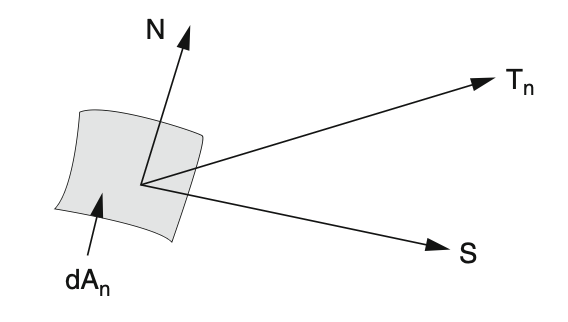
\includegraphics[width=0.8\linewidth]{./figures/f2_4.png}
  \caption{Differential surface element.}
  \label{fig:f2_4}
\end{figure}

The tangential component $\sigma_{ns}$ is
\begin{align*}
  \sigma_{nn} = \left| \Vec{S} \right| &= \Vec{T}_n  \cdot \Vec{s}\\
                                       &= T_i \Vec{e}_i \cdot \Vec{s} \\
                                       &= T_i s_i \\
                                       &= \sigma_{ji} n_j s_i
.\end{align*}
where
\begin{equation*}
  s_i = \Vec{e}_i \Vec{s}
.\end{equation*}

Often it is easy to calculate $\sigma_{ns}$ using the Pythagorean theorem as
\begin{equation*}
  \sigma_{ns} = \sqrt{T_i T_i - \sigma^2_{nn}}
.\end{equation*}

One is also able to resolve $N$ and $S$ into Cartesian components using $(k)$ to designate the axes as
\begin{align*}
  \sigma_{nn(k)} = \Vec{N} \cdot \Vec{e}_k &= \sigma_{nn} \Vec{n} \cdot \Vec{e}_k  \\
  &= \sigma_{nn} n_k \\
  &= \sigma_{ji} n_j n_i n_k, \quad k = 1,2,3
.\end{align*}

For $\sigma_{ns}$ subtraction gives
\begin{equation*}
  \sigma_{ns(k)} = T_k - \sigma_{nn(k)} \quad k = 1,2,3
\end{equation*}
which may also be written as
\begin{equation*}
  \sigma_{ns(k)} = \sigma_{jk} n_j - \sigma_{ji} n_j n_i n_k = \left( \delta_{ki} - n_i n_k  \right) \sigma_{ji} n_j
.\end{equation*}

\subsubsection{Dyadic Representation of Stress}
One is able to view the stress tensor as a vector-like quantity with a magnitude and associated direction(s) specified by unit vectors.
The \textit{dyadic} is such a representation.
We write the stress tensor or stress dyadic as
\begin{align*}
  \Vec{\sigma} &= \sigma_{ij} \Vec{e}_i \Vec{e}_j \\
               &= \sigma_{11} \Vec{e}_1 \Vec{e}_1 + \sigma_{12} \Vec{e}_1 \Vec{e}_2 + \sigma_{13} \Vec{e}_1 \Vec{e}_3 + \sigma_{21} \Vec{e}_2 \Vec{e}_1 + \sigma_{22} \Vec{e}_2 \Vec{e}_2 + \sigma_{23} \Vec{e}_2 \Vec{e}_3 + \sigma_{31} \Vec{e}_3 \Vec{e}_1 + \sigma_{32} \Vec{e}_3 \Vec{e}_2 + \sigma_{33} \Vec{e}_3 \Vec{e}_3
\end{align*}
wherein the double vectors are called \textit{dyads}.
The corresponding tractions are evaluated by an operation analogous to the dot product:
\begin{equation*}
  \Vec{T}_i = \Vec{\sigma} \cdot \Vec{e}_i = \sigma_{ij} \Vec{e}_j
.\end{equation*}

Similarly, the normal and tangential components of the traction $\Vec{T}_n$ on a plane defined by normal $\Vec{n}$ are
\begin{align*}
  \sigma_{nn} &= \Vec{\sigma} \cdot \Vec{n} \cdot \Vec{n} \\
  &= \Vec{T}_n \cdot \Vec{n} \\
  &= \sigma_{ij} n_i n_j
\end{align*}
and
\begin{align*}
  \sigma_{ns} &= \Vec{\sigma}\cdot \Vec{n} \cdot \Vec{s} \\
  &= \Vec{T}_n \cdot \Vec{s} \\
  &= \sigma_{ij} n_i s_j
.\end{align*}
